\chapter{Resultados y Conclusiones}
\label{ch:conclusiones}
Este capítulo recoge los resultados obtenidos de la realización del proyecto, siguiendo las directrices y procedimientos marcados en el capítulo \ref{ch:metodologia}. En este capítulo, se describirán los resultados siguiendo los mismos epígrafes que el capítulo \ref{ch:metodologia}, para así ver de forma más clara cómo ha progresado cada parte de la metodología.\\

Tras el análisis de la misma y una serie de conclusiones positivas y negativas del proyecto, se prosigue con una serie de propuestas de mejora de cara a sucesivas iteraciones del proyecto.

\section{Desarrollo de la metodología}
\subsection{El equipo}
A lo largo del proyecto, el equipo se ha visto afectado por numerosos cambios repentinos y no previstos, que incluyen bajas e incorporaciones de nuevos miembros. Esto requería un esfuerzo adicional de adaptación del nuevo compañero o compañera, al que había que poner en situación del proyecto, conocer sus cualidades y puntos fuertes, etc.\\

En la imagen \ref{asistencias} se puede ver un gráfico de número de asistencias de los miembros del equipo a las reuniones. Ha de tenerse en cuenta que no todos los miebros del equipo entraron al principio.\\

\begin{figure}
    \centering
    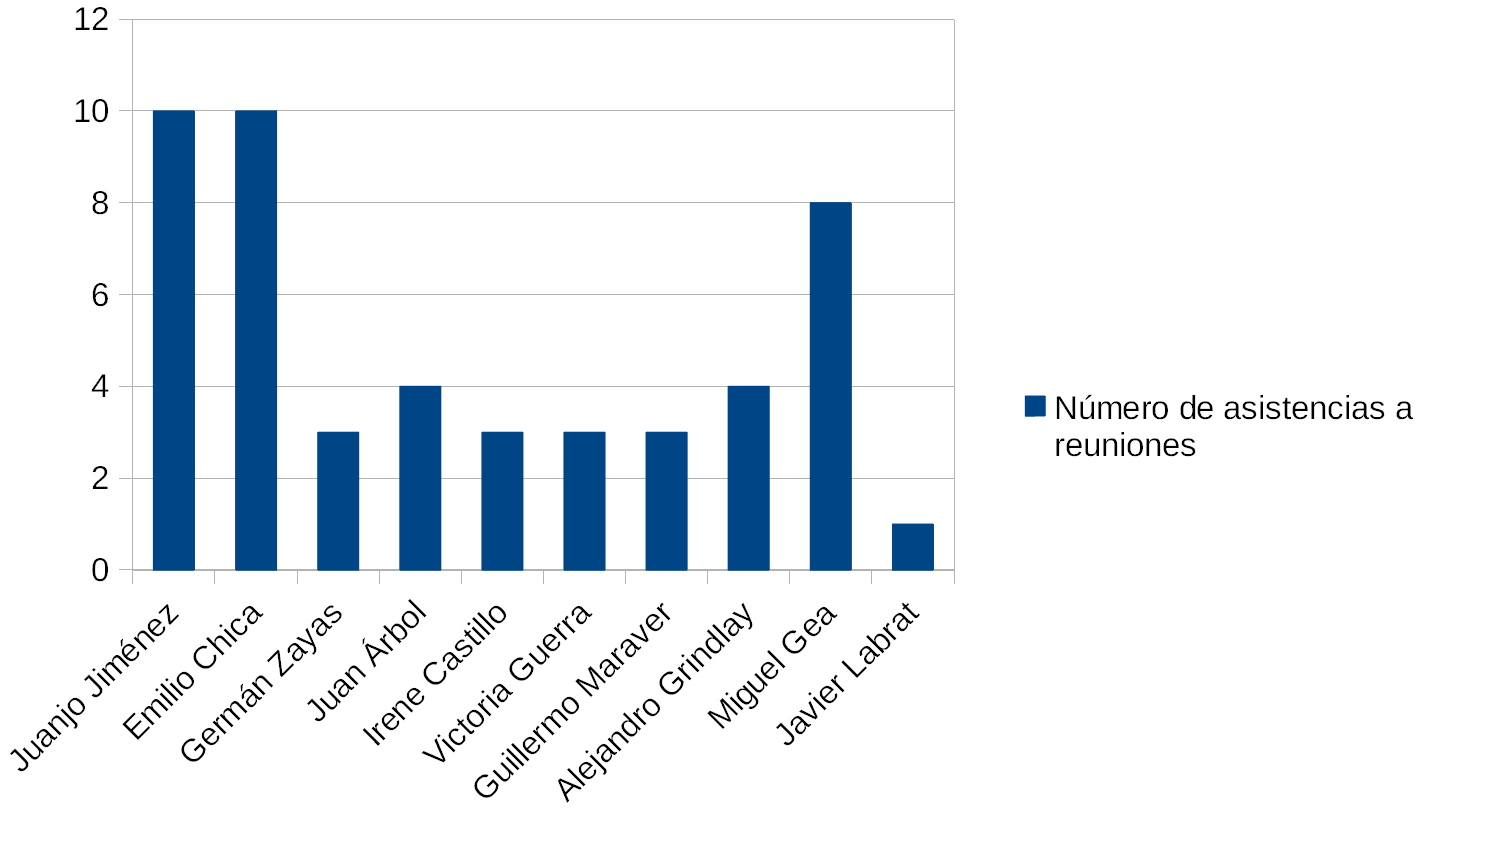
\includegraphics[scale=0.8]{asistencias}
    \caption{Gráfico de asistencias de los integrantes a las reuniones}
    \label{asistencias}
\end{figure}

Debido a la amplia disparidad de tiempo disponible que tenía cada uno de los integrantes, la coordinación no fue del todo exitosa. Surgieron numerosos contratiempos de planificación de reuniones. Esto afectó en cierta medida a la temporización del proyecto, que se ve con más detalle en el siguiente apartado.\\

Para lograr una mejor coordinación, este tipo de proyectos requieren de más dedicación y coordinación. Se ha visto que acciones como encontrar un día de la semana común para organizar reuniones semanales ayuda en gran medida a la organización. En caso de que no pueda asistir alguien en alguna ocasión a las reuniones, las actas de reunión son una buena forma de que los ausentes se pongan al día en lo que se ha avanzado.\\

Durante el proyecto, se realizaron una serie de actas más básicas que recogían lo esencial que fue tratado en la reunión, pero en el anexo se puede encontrar una propuesta de plantilla más elaborada que permite organizar y controlar mejor los asuntos del proyecto, como las tareas planificadas, objetivos para siguientes reuniones, etc.

\subsection{Temporización}
La planificación inicial que se realizó sufrió grandes variaciones a lo largo del curso. Debido a varios retrasos y dificultades para la organización de las reuniones, se sufrían retrasos de varias semanas hasta poder encontrar puntos comunes en los que la mayoría de personas del equipo se podían reunir. En la tabla \ref{temporizacion} se puede consultar la temporización del proyecto.\\

\begin{table}
    \begin{center}
        \begin{tabular}{|p{5cm}|p{3cm}|p{3cm}|}
            \hline
                \rowcolor{Gray}\multicolumn{1}{|c|}{\textbf{Hito o tarea}}
                & \multicolumn{1}{|c|}{\textbf{Fecha de inicio}}
                & \multicolumn{1}{|c|}{\textbf{Fecha de finalización}}\\
            \hline
                Reuniones iniciales de presentación, explicación y creación de seminarios & Principios de noviembre de 2016 & Finales de diciembre de 2016 \\
            \hline
                Creación de seminarios y design thinking & Principios de febrero de 2017 & Finales de marzo de 2017\\
            \hline
                Realización de los seminarios de tecnologías y Design Thinking & Finales de marzo de 2017 & Principios de abril de 2017 \\
            \hline
                Comienzo del desarrollo del proyecto y tareas asignadas a cada miembro & Principios de mayo de 2017 & Principios de junio de 2017 \\
            \hline
                Reuniones finales de testeo y coordinación de defensas de TFGs & Principios de junio de 2017 & Mediados de junio de 2017 \\
            \hline
                Finalización de la documentación de mi proyecto & Principios de julio de 2017 & Finales de noviembre de 2017 \\
            \hline
        \end{tabular}
        \caption{Temporización general del proyecto}
        \label{temporizacion}
    \end{center}
\end{table}

\subsection{Seminarios y divulgación}
Una vez expuesto el catálogo de posibles técnicas de creatividad y generación de ideas, se optó por realizar un \textbf{seminario informativo de tecnologías emergentes}, otro sobre \textbf{técnicas de creatividad}, seguido de un proceso creativo de \textit{Design Thinking} para que todos aportaran ideas y conceptos que nos servirían para dar forma a nuestro sistema a desarrollar. En el anexo \ref{sec:designthinking} podrá encontrar una \textbf{lista de todas las ideas} que se obtuvieron, clasificadas de la siguiente manera:

\begin{itemize}
    \item Ideas
    \item Objetivos
    \item Limitaciones
    \item Aspectos positivos
\end{itemize}

Más adelante se realizó otra sesión de Design Thinking debido a que hubo algunas ausencias en la primera reunión, y sirvió para \textbf{afianzar todo lo visto} en la primera y proceder con ello al desarrollo del producto software, que se detalla en el capítulo \ref{ch:desarrollo}.\\

En el anexo puede encontrar disponible las actas de reunión realizadas durante este primer año de vida del proyecto.

\subsection{Comunicación}
Como detalle final de la gestión de la comunicación, en la tabla \ref{canalescomunicacion} se puede ver las valoraciones dadas tras su uso a los distintos canales de comunicación que utilizamos entre los miembros del equipo.

\begin{table}
    \begin{center}
        \begin{tabular}{|l|p{3cm}|p{5cm}|}
            \hline
                \rowcolor{Gray}\multicolumn{1}{|c|}{\textbf{Canal}}
                & \multicolumn{1}{|c|}{\textbf{Utilidad}} & \multicolumn{1}{|c|}{\textbf{Valoración}} \\
            \hline
                E-mail & Usado en las primeras semanas & No es recomendable, debido a que no siempre se comprueba el correo electrónico con regularidad y no se sabe si alguien lo ha leido. \\
            \hline
                WhatsApp \cite{whatsapp} & Utilizado durante todo el proyecto & Aplicación de mensajería más utilizada, respuesta casi inmediata y mayor rapidez de comunicación. \\
            \hline
                Slack \cite{slack} & Utilizado al final del proyecto & Es una plataforma muy utilizada por empresas y equipos de desarrollo, con numerosas funcionalidades de comunicación entre miembros que agilizan bastante la comunicación. \\
            \hline
        \end{tabular}

        \caption{Canales de comunicación empleados y valoración de los mismos}
        \label{canalescomunicacion}
    \end{center}
\end{table}

A pesar de las ventajas que aportaba Slack, finalmente no se utilizó de forma global en el equipo, sino únicamente por un grupo reducido de personas del mismo. El motivo es que requiere de una pequeña introducción al resto de compañeros para que conozcan los fundamentos básicos de su funcionamiento, pero no se realizó dicha clase introductoria.\\

A pesar de esto, se recomienda el uso de Slack y para ello, se sugiere que al empezar un nuevo proyecto, una de las primeras tareas sea la de enseñar a usarlo y fomentarlo.

\subsection{Dependencias entre miembros del equipo}
Nos encontramos con los siguientes ejemplos de tareas en las que hemos encontrado sinergias, es decir, que gracias a la colaboración mutua, el resultado obtenido es mejor que haberlo hecho por separado:

\begin{itemize}
    \item La propia \textbf{implementación de las plataformas} colaborando con mi compañero Emilio consiguió que el software propuesto presentara una funcionalidad más rica y completa que haberlo hecho por separado.
    \item Germán aportó sinergias en casi todas las líneas de trabajo, ya que su tarea (\textbf{diseño de la identidad corporativa}) es aplicable no solo al software, sino también al marketing.
    \item Entre Germán y Juan hubo colaboración para confeccionar el diseño de la \textbf{página web de presentación del proyecto}, así como la creación de sus contenidos.
    \item Javier, con su proyecto ya terminado, sirvió como \textbf{prueba de concepto}, al permitir incorporar su proyecto al futuro sistema que se va a diseñar para demostrar al público objetivo las capacidades de SmartU.
\end{itemize}

Pero también es cierto que hubo ciertos problemas a lo largo del curso que impidieron la aprición de más sinergias. Principalmente los problemas fueron la falta de tiempo para que algunos miembros pudieran hacer sus tareas, y la tardía definición de todos los conceptos del proyecto y la necesidad de la aplicación móvil, que en un principio no quedaba clara cual podía ser tu utilidad y diferenciación.\\

Esta experiencia nos hace ver que este tipo de proyectos requieren de más dedicación de la que se pensaba. Al ser una primera experiencia piloto, no teníamos del todo claro lo que podía pasar, pero ello nos servirá para que en los años siguientes el proceso mejore.

\section{Valoración personal}
Tras todos estos meses de trabajo, la experiencia adquirida es de enorme valor. Aunque ha habido contratiempos, no se puede negar que se han hecho importantes progresos en el inicio de este proyecto. Se ha conseguido formar un equipo de trabajo de diferentes especialidades y se ha podido obtener de todos ellos mucha información, además de aprender a aprovechar los puntos fuertes de cada uno para realizar partes de este proyecto.\\

Personalmente, quiero destacar que ha sido muy revelador el haber compartido trabajo con personas de otras disciplinas y estudios. Tras muchos años trabajando en equipo con compañeros informáticos, nos acostumbramos demasiado y no sabemos tratar con personas que no tienen los mismos conocimientos que nosotros. Junto a esto, ha sido positivo el haber podido coordinar en la medida de lo posible a todos para poder reunirnos sin alterar la rutina y obligaciones diarias de cada uno de los miembros.\\

El trabajo en equipo nunca es fácil, ya que requiere de un gran compromiso por parte de todos los integrantes para que pueda haber un cierto nivel de éxito. No importa que sea poco al principio si se consigue poner la primera piedra de un proyecto que se espera que a largo plazo se refine más. El hecho de poder coordinar (en mayor o menor medida) a estudiantes de diferentes disciplinas de conocimiento pone en valor lo enriquecedor que supone un trabajo que recibe apoyo de distintos puntos de vista.\\

Por ello, espero que estas páginas y las de los proyectos del resto de mis compañeros sean en el futuro de gran utilidad y permitan que en el futuro, los proyectos multidisciplinares sean una parte más dentro de la vida universitaria, y que los estudiantes no tengan miedo a adentrarse en un proyecto en equipo. Nadie dijo que fuese algo fácil, pero no es imposible.\\

Debido a que la tarea de gestión del proyecto ha sido más laboriosa y ha requerido más tiempo y esfuerzo para llevarla a cabo, por el hecho de organizar y sincronizar a los integrantes del equipo, como consecuencia de ello, mi tarea de desarrollo de software se ha visto mermada y reducida en tiempo y recursos para poder completarla.\\

De esta situación, puedo afirmar que la tarea de gestión alberga una dedicación y complejidad que haría más recomendable que la persona a cargo de la misma, no dedique su tiempo y esfuerzo a otras tareas diferentes, ya que es posible que, o no realice una correcta gestión y atienda a la organización de todos los miembros, o sus otras tareas sean de una calidad reducida.

\section{Objetivos conseguidos}
Aunque el proyecto ha tenido sus problemas, quiero destacar que se han logrado varios objetivos gracias al esfuerzo y trabajo de todos los compañeros. En primer lugar, hemos creado una primera versión de una metodología de trabajo en equipo que confiamos en que mejore con los años. A modo de experimento, hemos aplicado nuestros actuales conocimientos y hemos visto las fortalezas y debilidades de esta forma de trabajar.

\subsection{Productos creados}
Es importante que, como gestor del proyecto, además de desarrollador, ponga en valor todo lo que se ha ido creando, ya que, aun incompletos, existen una serie de \textit{deriverables} que sirven como base para completar en el futuro.\\

\subsubsection{Software}
Tenemos las primeras versiones de dos entregables importantes: la \textbf{app web} y la \textbf{app móvil} de mi compañero Emilio. De esta última se puede ver más detalle y explicación en el correspondiente trabajo de fin de grado \textit{``SmartU la red social - La Universidad conectada a la Ciudad sostenible''}. Es cierto que ha habido ciertas complicaciones debido a imprevistos y falta de tiempo, y que no he podido crear un producto con un 100\% de calidad, pero la idea de un desarrollo ágil es ir mejorando con el tiempo lo existente e incorporarle nuevas funcionalidades.

\subsubsection{Diseño gráfico}
Nuestro compañero Germán, en su proyecto \textit{La Universidad conectada a la Ciudad Sostenible, propuesta de espacio coworking de ideas y servicios}, ha elaborado un plan de diseño gráfico e identidad visual para la marca, que aporta modernidad y un diseño atractivo que servirá para atraer a los estudiantes y fomentar el uso de SmartU.

Aunque de momento el proyecto no ha aplicado esta guía de estilo, ya está creada, de modo que en sucesivas iteraciones se puede aplicar y empezar a usar.

\subsubsection{Audiovisuales}
Irene, con su proyecto \textit{Nuevos modelos de producción documental: Prototipo de video inmersivo de promoción del proyecto interdisciplinar SmartU}, ha ideado una estrategia de promoción muy innovadora y adaptada a las tecnologías presentes hoy en día, como son los videos en 360º. La promoción es muy importante para darse a conocer, e impresionar a los posibles usuarios de SmartU puede conseguir un gran éxito.

\section{Mejoras para el futuro}
El proyecto cuenta con diversas líneas de trabajo, en las que todavía queda espacio para mejoras y ampliación de su desarrollo. En un principio se supo que no iban a quedar todas las líneas finalizadas en su primer año de vida, así que las personas que decidan continuarlo se encargarán de seguir completándolo.

\subsection{Mejoras de la gestión}
El equipo multidisciplinar recomienda que se sigan las directrices mencionadas en el capítulo de la metodología de trabajo, y animamos a que se perfeccione y corrija todo lo que se vea que requiere mejora, para conseguir mejores resultados en años venideros.\\

A lo largo de este capítulo se han ido viendo los problemas derivados de la gestión que han ido surgiendo, y posibles mejoras al respecto. Esta serie de mejoras han de solventarse desde el principio, ya que de no hacerlo, serían recurrentes y volveríamos a encontrarnos con los mismos problemas:

\begin{itemize}
    \item La organización desde el principio es muy importante en un equipo tan heterogéneo. Hay que estar preparado para el cambio, incorporaciones y bajas de miembros del equipo.
    \item Relacionado con lo anterior, la comunicación juega un papel fundamental en la organización, por lo que una plataforma adecuada desde el principio mejoraría este aspecto.
    \item El compromiso personal de todos. Este tipo de proyectos requiere de mayor esfuerzo por la coordinación con otras personas y ajuste y cuadre de sus agendas.
    \item Este proyecto tenía un ámbito muy ambiuo y poco definido debido a las circunstancias. El proyecto es muy novedoso y se basa en el estudio de una metodología de trabajo. Es importante que desde el principio se defina muy bien los objetivos que se quieren realizar y ajustarse a dicho plan.
\end{itemize}

\subsection{Mejoras del desarrollo}
Existen numerosas mejoras que se pueden realizar en lo que respecta a mi línea de trabajo. Para consultar las posibles mejoras de otras líneas, consulta los TFGs de mis compañeros de equipo multidisciplinar. He confeccionado la siguiente lista en base a mi experiencia y trabajo realizado:

\begin{itemize}
    \item Debido a problemas de tiempo, mi proyecto no está \textbf{integrado completamente} con la aplicación móvil de mi compañero Emilio. Ambas aplicaciones se han construido bajo una misma lista de requisitos y funcionalidades, pero es necesario integrar ambas plataformas bajo una misma API para que lo que se haga en una se refleje en la otra, y viceversa.
    \item Partiendo del punto anterior, en la aplicación web \textbf{faltan diversas funcionalidades} que sí están presentes en la móvil, como es el caso del chat individual entre usuarios.
    \item Aunque la aplicación web presenta un diseño adaptable que permite su visualización en todos los formatos de pantalla, sería interesante estudiar el llevarlo a \textbf{otras plataformas móviles} como iOS o Windows 10 Mobile, de forma nativa.
    \item La \textbf{gestión del contenido multimedia} es mejorable en la aplicación web, pudiendo implementar una funcionalidad similar a la existente en la aplicación móvil.
    \item Se pueden realizar \textbf{mejoras en las funcionalidades existentes} actualmente. Los proyectos pueden tener más complejidad o información que mostrar al usuario, así como mejoras en la funcionalidad de vacantes y avances.
    \item La aplicación web contiene \textbf{soporte para múltiples idiomas}. Aunque de momento solo cuenta con el inglés y el español, siempre se pueden añadir más para que más personas puedan hacer uso de SmartU.
\end{itemize}
